\subsection{Graph Analytics}
%\help{In this case, the two main highlights are that Finch can do arbitrary operators (i.e. choose), and that Finch can do early break, and also the different loop orders and multiple outputs. We may need to explain a little bit about what push pull is. For bellman, the main point is that we need multiple outputs, sparse inputs, masks, and sparse outputs with differing formats at differing points.}

We used Finch to implement both Breadth-first search (BFS) and Bellman-Ford single-source shortest path.
%
Our BFS implementation and graphs datasets are taken from Yang et al.~\cite{yang_implementing_2018}, including both road networks and scale-free graphs (bounded node degree vs. power law node degree).

%road networks, characterized by bounded node degrees and long diameters, and scale-free graphs, where node degree distribution follows a power-law distribution and diameters are short.

Direction-optimization~\cite{beamer_direction-optimizing_2012} is crucial for achieving high BFS performance in such scenarios, switching between push and pull traversals to efficiently explore graphs.
%
Push traversal visits the neighbors of each frontier node, while pull traversal visits every node and checks to see if it has a neighbor in the frontier. 
%
The advantage of pull traversal is that we may terminate our search once we find a node in the frontier, saving time in the event the push traversal were to visit most of the graph anyway. 
%
Early break is the critical part of control flow in this algorithm, though the algorithms also require different loop orders, multiple outputs, and custom operators.

Figure~\ref{fig:graph_result} compares performance to Graphs.jl, a Julia library, and the LAGraph Library, which implements graph algorithms with sparse linear algebra using GraphBLAS~\cite{mattson_lagraph_2019}.
%
For the BFS algorithm, direction-optimization notably enhances performance for scale-free graphs. 
%
Although GraphBLAS uses hardwired optimizations, Finch is competitive. 
%
On Bellman-Ford (with path lengths and shortest-path tree), Finch's support for multiple outputs, sparse inputs, and masks leads to superior performance over GraphBLAS (average speedup of 3.53). 
%
We did not include GAP-road as it timed out. %speedup is arith-mean
%
In Appendix B, we display the code for BFS and Bellman-Ford in Finch (57 and 50 LOC) and LAGraph (215 and 227 LOC), and invite readers to compare the clarity of the algorithms.
 
\begin{figure}[b]
    \begin{minipage}{0.33\linewidth}
    \begin{minted}{julia}
    V = Tensor(Dense(Element(false)))
    P = Tensor(Dense(Element(0)))
    F = Tensor(SparseByteMap(Pattern()))
    _F = Tensor(SparseByteMap(Pattern()))
    A = Tensor(Dense(SparseList(Pattern())))
    AT = Tensor(Dense(SparseList(Pattern())))

    function bfs_push(_F, F, A, V, P)
      @finch begin
        _F .= false
        for j=_, k=_
          if F[j] && A[k, j] && !(V[k])
            _F[k] |= true
            P[k] <<choose(0)>>= j
          end
        end
        return _F
      end
    end

    \end{minted}
\end{minipage}%
\begin{minipage}{0.33\linewidth}
    \begin{minted}{julia}
    function bfs_pull(_F, F, AT, V, P)
      p = ShortCircuitScalar{0}()
      @finch begin
        _F .= false
        for k=_
          if !V[k]
            p .= 0
            for j=_
              if F[follow(j)] && AT[j, k]
                p[] <<choose(0)>>= j
              end
            end
            if p[] != 0
              _F[k] |= true
              P[k] = p[]
            end
          end
        end
        return _F
      end
    end
    \end{minted}
\end{minipage}%
\begin{minipage}{0.33\linewidth}
  \begin{minted}{julia}
  _D = Tensor(Dense(Element(Inf)), n)
  D = Tensor(Dense(Element(Inf)), n)
  function bellmanford(A, _D, D, _F, F)
    @finch begin
    F .= false
    for j = _
      if _F[j]
        for i = _
          let d = _D[j] + A[i, j]
            D[i] <<min>>= d
            F[i] |= d < _D[i]
          end
        end
      end
    end
  end
\end{minted}
\end{minipage}
\caption{Graph Applications written in Finch. Note that parents are calculated separately for Bellman-Ford. The $choose(z)$ operator is a GraphBLAS concept which returns any argument that is not $z$.}\label{fig:graph_listing}
\end{figure}

\begin{figure}[t]
	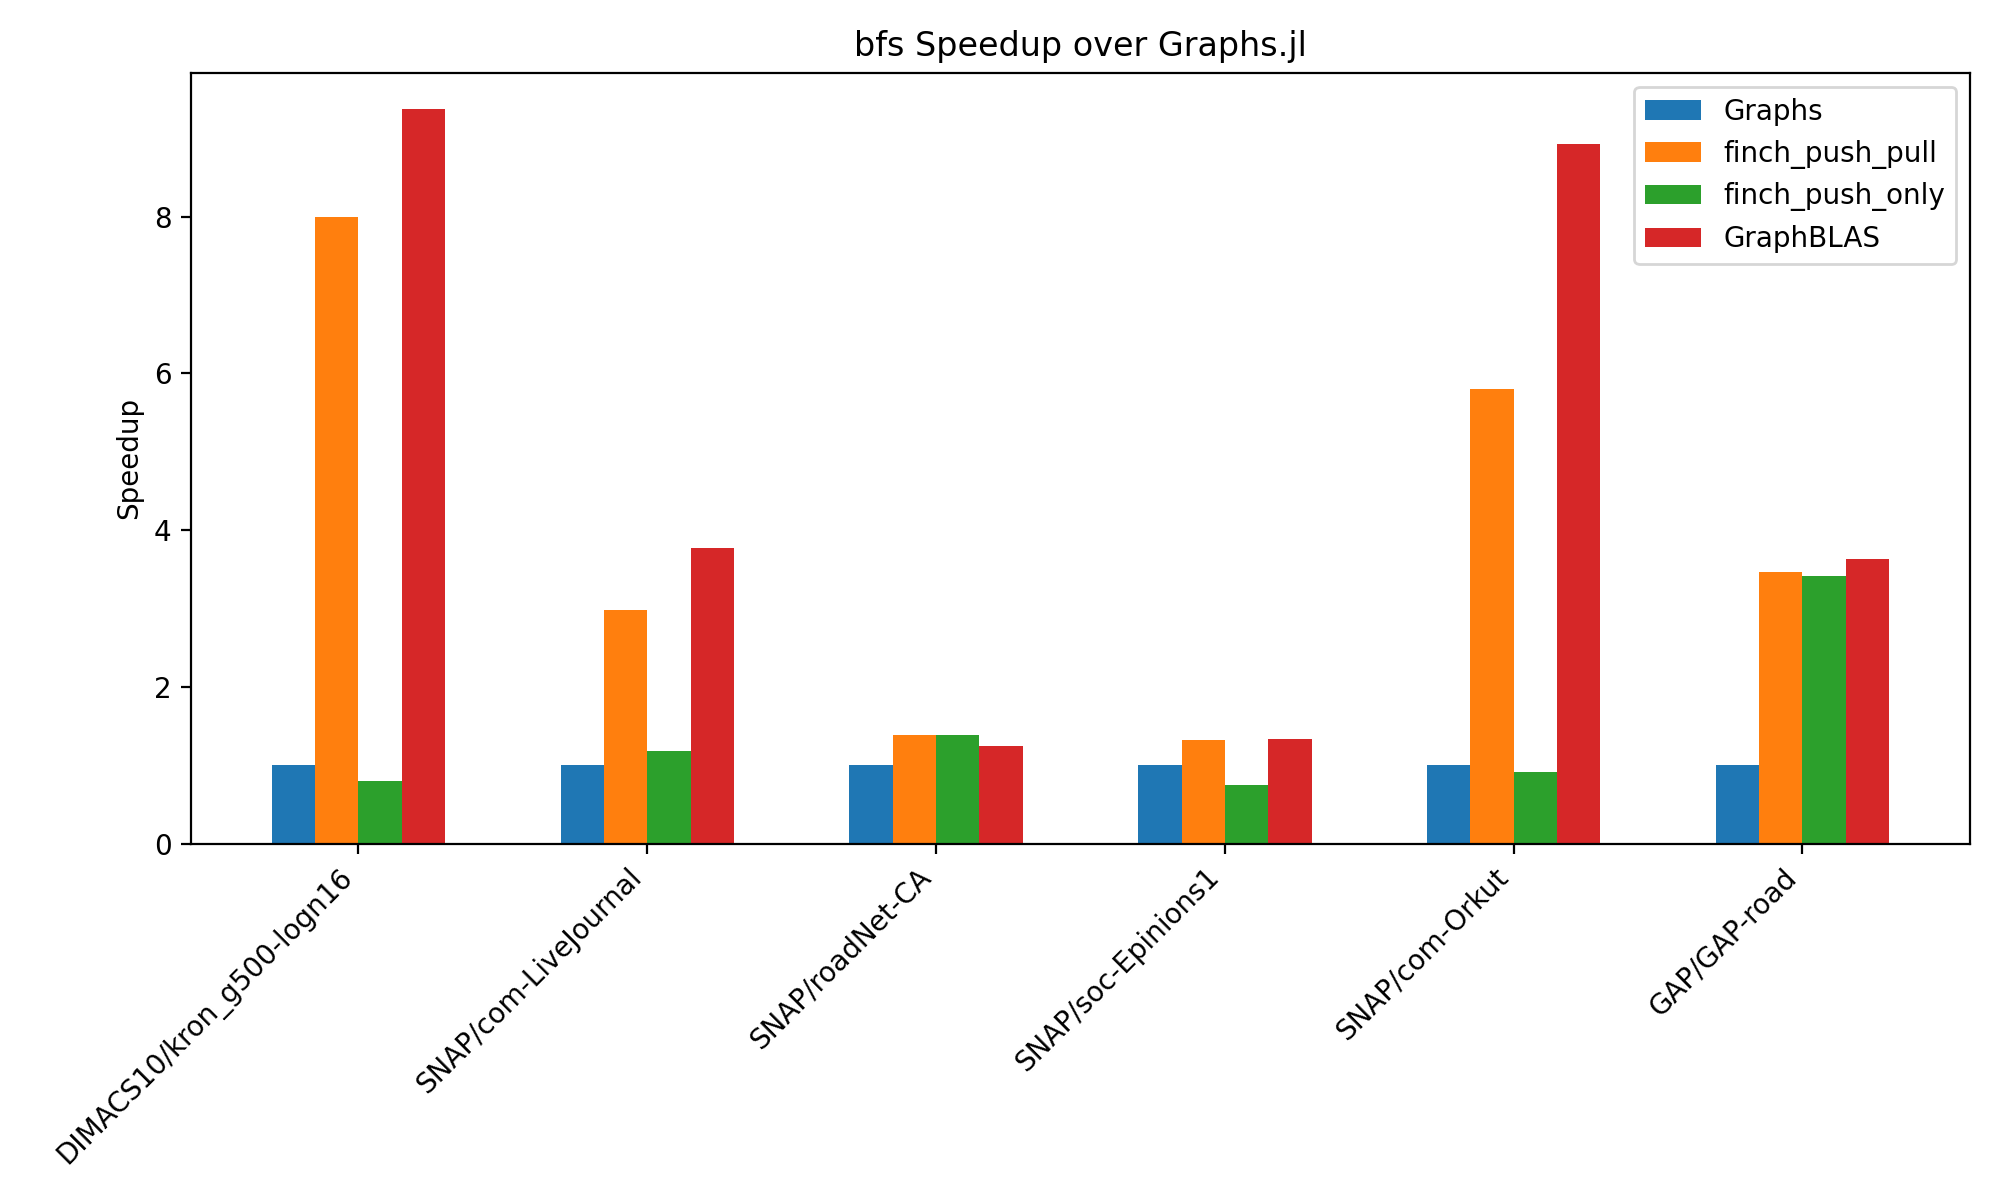
\includegraphics[width=0.5\linewidth]{bfs_speedup_over_graphs.jl.png}%
	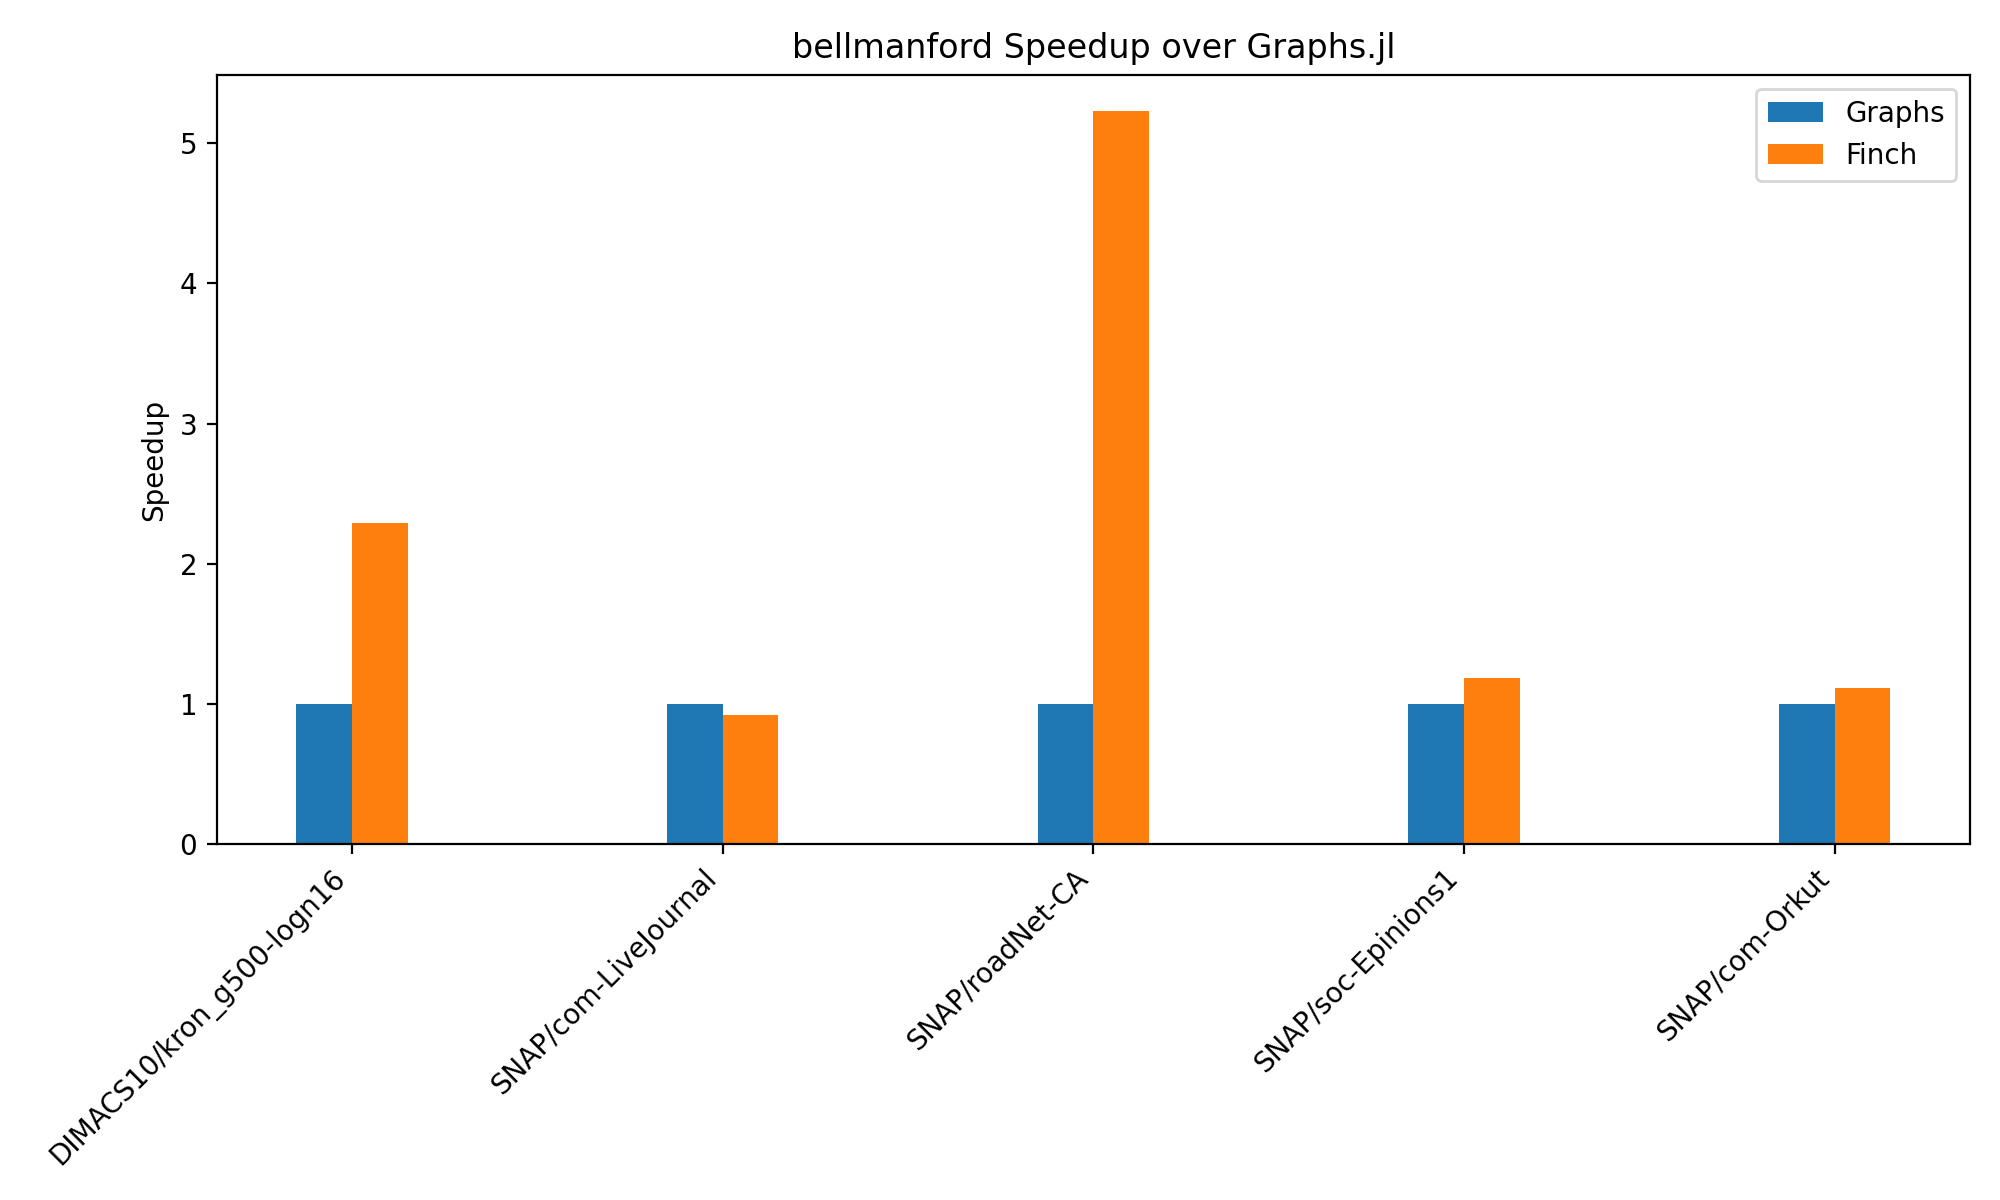
\includegraphics[width=0.5\linewidth]{bellmanford_speedup_over_graphs.jl.png}
    \vspace{-12pt}
    \caption{Performance of graph apps across various tools. finch\_push\_only exclusively utilizes push traversal, while finch\_push\_pull applies direction-optimization akin to GraphBLAS. Finch's support for push/pull traversal and early break facilitates direction-optimization. Among GraphBLAS's five variants for Bellman-Ford, we selected LAGraph\_BF\_full1a, consistently the fastest with our graphs.}
     \label{fig:graph_result}
\end{figure}